\exo7id{7582}
\titre{Calcul d'intégrales rationnelles}
\theme{}
\auteur{mourougane}
\date{2021/08/10}
\organisation{exo7}
\contenu{
  \texte{On considère la fonction méromorphe $f(z)=\frac{z^2}{1+z^4}$ sur $\Cc$.}
\begin{enumerate}
  \item \question{Montrer que $zf(z)$ a une limite quand $|z|$ tend vers $+\infty$.}
  \item \question{Montrer que $\int_{-\infty}^{+\infty}\frac{x^2}{1+x^4}dx$ converge.}
  \item \question{Déterminer les pôles de $f$ contenus dans le demi-plan $\mathbb{H}:=\{z\in\Cc, Im(z)>0\}$ et leurs résidus.}
  \item \question{En intégrant sur le chemin $\Gamma$ défini par
 $$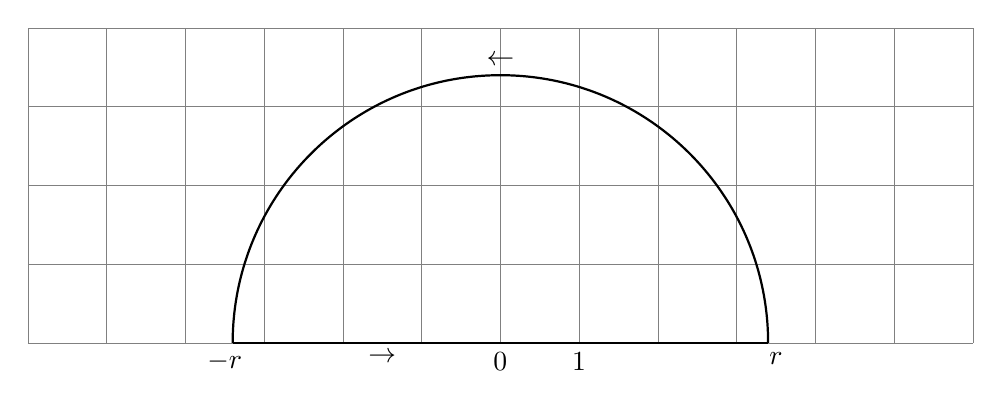
\begin{tikzpicture}
\draw[help lines, step=1, very thin] (-6,0) grid (6,4);
\draw[shift={(3.4,0)}, thick] (6:0) arc (0:180:3.4); \draw (0,3.4) node[above]{$\leftarrow$} ;
\draw[thick] (-3.4,0) -- (3.4,0) ;
\draw (0,0) node[below]{$0$} ;
\draw (3.5,0) node[below]{$r$} ;\draw (-3.5,0) node[below]{$-r$} ;\draw (-1.5,0) node[below]{$\to$} ;
\draw (1,0) node[below]{$1$} ;
\end{tikzpicture}$$
montrer que 
$$\int_{-r}^rf(x)dx+\int_{\partial(\Delta_r\cap\mathbb{H})} f(z)dz=2i\pi\sum_{c\in\mathbb{H}}Res_c(f).$$}
  \item \question{Montrer que $$\int_{-\infty}^{+\infty}\frac{x^2}{1+x^4}dx=\frac{\pi}{\sqrt{2}}.$$}
\end{enumerate}
\begin{enumerate}

\end{enumerate}
}